\documentclass[aspectratio=169]{beamer}
\mode<presentation>
\usepackage{dsfont}
\usepackage{exscale}
\usepackage[ruled]{algorithm2e} % must be loaded after natbib
\usepackage{dsfont}
\usepackage{mdwlist}
\usepackage{amsmath}
\usepackage{lmodern}
\usepackage{booktabs}
\usepackage{subfigure}
\usepackage{xspace}

\usetheme[height=0pt]{Rochester}
%\useoutertheme[footline=empty]{miniframes}
\useinnertheme{circles}
\setbeamercolor{math text}{fg=red}
\setbeamercolor{frametitle}{fg=blue}
%\setbeamercolor{framesubtitle}{fg=blue}
\setbeamertemplate{frametitle}
{
\begin{centering}
\insertframetitle\par
\insertframesubtitle\par
\end{centering}
}
\beamertemplatenavigationsymbolsempty

\setbeamertemplate{caption}{\raggedright\insertcaption\par} % remove "Figure" in captions

\newcommand{\purple}{\color{purple}}
\newcommand{\black}{\color{black}}
\newcommand{\green}{\color{green}}
\newcommand{\red}{\color{red}}

\newcommand*{\allsp}{\ensuremath{\mathbb{S}}\xspace}
\newcommand*{\Sam}{{\cal S}\xspace}
\newcommand*{\range}{\mathcal{R}\xspace}
\newcommand*{\expectation}{\mathbb{E}\xspace}
\newcommand*{\indicator}{\mathds{1}\xspace}
\newcommand*{\family}{{\cal F}\xspace}
\newcommand*{\domain}{{\cal D}\xspace}
\newcommand*{\Rade}{\mathsf{R}\xspace}
\newcommand*{\prob}{\pi\xspace}

%% high level macros
\newcommand*{\betw}{\ensuremath{\mathsf{b}}\xspace}
\newcommand*{\tbetw}{\ensuremath{\tilde{\betw}}\xspace}
\newcommand{\dist}{\ensuremath{d}\xspace}
\newcommand{\dep}{\ensuremath{\delta}\xspace}
\newcommand{\paths}{\ensuremath{\sigma}\xspace}
\newcommand{\pred}{\ensuremath{P}\xspace}
\newcommand{\sssp}{\ensuremath{\textsc{sssp}}\xspace}
\renewcommand{\dag}{\ensuremath{\textsc{dag}}\xspace} % no need for daggers
\newcommand{\spath}{\ensuremath{\mathcal{S}}\xspace}
\newcommand{\allspath}{\ensuremath{\mathbb{S}\xspace}}

\newtheorem{Claim}{Claim}

%% slide number
\addtobeamertemplate{navigation symbols}{}{%
    \usebeamerfont{footline}%
    \usebeamercolor[fg]{footline}%
    \hspace{1em}%
    \insertframenumber/\inserttotalframenumber
}

\title{Centrality Measures on Big Graphs\\Exact, Approximated, and Distributed Algorithms}
\author[Bonchi, De-Francisci-Morales, Riondato]{Francesco Bonchi\inst{1} \and
Gianmarco De-Francisci-Morales\inst{2} \and Matteo Riondato\inst{3}}
\date[WWW'16]{WWW'16 -- Montr\'eal, April 11--15, 2016}
  \institute[ISI, Qatar Computing Research Institute, TwoSigma]{
  \inst{1} ISI Foundation
  \and
  \inst{2} Qatar Computing Research Institute
  \and
  \inst{3} Two Sigma Investments
}

\begin{document}
\begin{frame}
  \titlepage
\end{frame}

\begin{frame}
  \frametitle{Notation}
  \begin{itemize}
    \item Graph $G=(V,E)$. $|V|=n$, $|E|=m$.
    \item All Shortest Paths (SPs) from node $s$ to node $t$: $\spath_{st}$.
    \item All shortest paths in the graph:
      $\allspath_G=\cup_{s,t}\spath_{st}$.
    \item Number of SPs from $s$ to $t$: $\paths_{st}=|\spath_{st}|$.
    \item Number of SPs from $s$ to $t$ that go through $w$: $\paths_{st}(w)$.
    \item Pair dependency of $(s,t)$ on $w$:
      $\dep_{st}(w)=\paths_{st}(w)/\paths_{st}$.
    \item Dependency of a node $s$ on another node $w$:
      $\dep_s(w)=\sum_{t \in V}\dep_{st}(v)$.
    \item Predecessors of a node $w$ in a shortest path DAG from source $s$:
      $\pred_s(w)$
    \item An edge $e$ is \emph{added} and \emph{removed} (addition and removal, no insertion, deletion)
    \item \ldots
  \end{itemize}
\end{frame}

\begin{frame}
  \frametitle{What vertices in a graph are important?}
  Betweenness centrality is one measure of vertex importance\\
  \quad Roughly, it is the fraction of Shortest Paths (SP) in a graph that go through a vertex
  \vfill
  Let $G=(V,E)$, $|V|=n$, $|E|=m$. The betweenness centrality of $v\in V$ is:
  \[
    \betw(v)=\underbrace{\frac{1}{n(n-1)}}_{\mbox{normalization}}\sum_{p_{uw}\in\mathbb{S}_G}
    \underbrace{\frac{\mathds{1}_{\mathcal{T}_v}(p_{uw})}{\sigma_{uw}}}_{\in [0,1]}
  \]
  where:
  \begin{itemize*}
    \item $\mathbb{S}_G$: set of all SPs in $G$
    \item $\mathcal{S}_{uw}$: set of all SPs from $u$ to $w$
      ($\mathcal{S}_{uw}\subseteq\mathbb{S}_G$,
      $|\mathcal{S}_{uw}|=\sigma_{uw}$)
    \item $\mathcal{T}_v$: $\{p\in\mathbb{S}_G ~:~ v\in\mathsf{Int}(p)\}$
  \end{itemize*}
\end{frame}

\begin{frame}
  \frametitle{How to compute betweenness centrality?}
  Na\"ive algorithm: All Pairs SP computation, followed by aggregation\\
  \quad Aggregation dominates runtime, $\Theta(n^3)$
  \vfill
  [Brandes 2001]: Perform aggregation after each Single-Source SP (SSSP) computation\\
  \quad Runtime: $O(nm)$ (unweighted $G$), $O(nm + n^2\log n)$ (weighted
  $G$)\\
  This is is still too much for graphs with $n=10^9$, $m=10^10$
  \vfill
  Possible solution: perform fewer SPs computations by sampling\\
  \quad We get approximate results, but that's OK!
  \vfill
  What kind of approximation do we want ? What should we sample and how much?
\end{frame}

\begin{frame}
  \frametitle{What kind of approximation do we want?}
  We want uniform quality guarantees on the approximations of all vertices
  \vfill
  Definition:\\
  \quad For $\varepsilon,\delta\in(0,1)$, an $(\varepsilon,\delta)$-approximation is
  a collection $\{\tilde{\betw}(v), v\in V\}$ such that
  \[
    \Pr(\exists v\in V ~:~ |\tilde{\betw}(v) -\betw(v)|>\varepsilon)<\delta
  \]
  $\varepsilon$ controls the accuracy, $\delta$ controls the confidence
  \vfill
  Trade-off: smaller $\varepsilon$ or $\delta$ $\Rightarrow$ higher number of
  samples $\Rightarrow$ slower runtime
\end{frame}

\begin{frame}
  \frametitle{How can one get an $(\varepsilon,\delta)$-approximation?}
  [Brandes and Pich, 2008]: only run SSSP and aggregation from a few sources
  \vfill
  \begin{algorithm}[H]
    \DontPrintSemicolon
    $r\leftarrow \frac{1}{\varepsilon^2}\left(\ln n + \ln 2 +
    \ln\frac{1}{\delta}\right)$ \texttt{// sample size}\;
    $\tilde{\betw}(v)\leftarrow 0$, for all $v\in V$\;
    \For(\texttt{// the exact algorithm would iterate over $V$}){$i\leftarrow 1,\dotsc,r$} {
      $v_i \leftarrow$ random vertex from $V$, chosen uniformly\;
      Perform single-source SP computation from $v_i$\;
      Perform partial aggregation, updating $\tilde{\betw}(u)$, $u\in V$,
      like in exact algorithm\;
    }
    Output $\{\tilde{\betw{v}}, v\in V\}$\;
  \end{algorithm}
  \vfill
  Theorem: The output is an $(\varepsilon,\delta)$-approximation
\end{frame}

\begin{frame}
  \frametitle{How do they prove it?}
  Start with bounding the deviation for a single vertex $v$ (Hoeffding bound):
  \[
    \Pr(|\tilde{\betw}(v)-\betw(v)|>\varepsilon)\le 2e^{-2r\varepsilon^2}
  \]
  \vfill
  Then take the union bound over $n$ vertices to ensure uniform converge\\
  \quad the sample size $r$ must be such that
  \[
    2e^{-2r\varepsilon^2}\le\frac{\delta}{n}
  \]
  That is, to get an $(\varepsilon,\delta)$-approximation, we need
  \[
    r\ge\frac{1}{2\varepsilon^2}\left(\ln n + \ln 2 +
    \ln\frac{1}{\delta}\right)
  \]
\end{frame}

\begin{frame}
  \frametitle{What is wrong with this approach?}
  1) We need
  \[
    r\ge\frac{1}{2\varepsilon^2}\left(\ln n + \ln 2 +
    \ln\frac{1}{\delta}\right)
  \]
  \begin{itemize}
    \item This is loose, due to the union bound and does not scale well (experiments)
    \item The sample size depends on $\ln n$. This is not the right
      quantity: not all graphs of $n$ nodes are equally ``difficult'': e.g., the $n$-star is ``easier'' than a random graph
  \end{itemize}
  The sample size $r$ should depend on a more-specific characteristic of the graph
  \vfill
  2) At each iteration, the algorithm performs a SSSP computation\\
  \quad Full exploration of the graph, no locality
\end{frame}

\begin{frame}
  \frametitle{How can we improve the sample size?}
  [R. and Kornaropoulos, 2014] present an algorithm that:
  \vfill
  1) uses a sample size which depends on the vertex-diameter, a characteristic
  quantity of the graph. The derivation uses VC-dimension
  \vfill
  2) samples SPs according to a specific, non-uniform distribution over
  $\mathbb{S}_G$. For each sample, it performs a single $s-t$ SP computation
    \begin{itemize}
      \item More locality: fewer edges touched than single-source SP
      \item Can use bidirectional search / A\textsuperscript{*},
        \ldots
      \end{itemize}
\end{frame}

\begin{frame}
  \frametitle{What is the algorithm?}
  \begin{algorithm}[H]
    \DontPrintSemicolon
    $\mathsf{VD}(G)\leftarrow$ vertex-diameter of $G$ \texttt{// stay
    tuned!}\;
    $r\leftarrow\frac{1}{2\varepsilon^2}\left(\lfloor\log_2(\mathsf{VD}(G)-2\rfloor)
    +1 + \ln(1/\delta)\right)$ \texttt{// sample size}\;
    $\tilde{\betw}(v)\leftarrow 0$, for all $v\in V$\;
    \For{$i\leftarrow 1\dotsc,r$}{
      $(u,v)\leftarrow$ random pair of different vertices, chosen
      uniformly\;
      $\mathcal{S}_{uv}\leftarrow$ all SPs from $u$ to $v$ \texttt{//
      Dijkstra, trunc.~BFS, \ldots}\;
      $p\leftarrow$ random element of $\mathcal{S}_{uv}$, chosen
      uniformly \texttt{// not uniform over $\mathbb{S}_G$}\;
      $\tilde{\betw}(w)\leftarrow \tilde{\betw}(w) + 1/r$, for all
      $w\in\mathsf{Int}(p)$ \texttt{// update only nodes along $p$}\;
    }
    Output $\{\tilde{\betw}(v), v\in V\}$
  \end{algorithm}
  Theorem: The output $\{\tilde{\betw}(v), v\in V\}$ is an
  $(\varepsilon,\delta$)-approximation
\end{frame}

\begin{frame}
  \frametitle{How can we prove the correctness?}
  We want to prove that the output $\{\tilde{\betw}(v), v\in V\}$ is an
  $(\varepsilon,\delta$)-approximation
  \vfill
  Let's apply the recipe!

  \begin{enumerate}
    \item  Define betweenness centrality computation as a expectation
      estimation problem (domain $\domain$, family $\family$, distribution
      $\prob$)
    \item Show that the algorithm efficiently samples according to $\prob$
    \item Show how to efficiently compute an upper bound to the VC-dimension\\
      \quad Bonus: show tightness of bound
    \item Apply the VC-dimension sampling theorem
  \end{enumerate}
\end{frame}

\begin{frame}
  \frametitle{How to define the expectation estimation task?}
  \begin{itemize}
    \item The domain $\domain$ is $\mathbb{S}_G$ (all SPs in $G$)\\
    \item The family is $\family=\{\mathds{1}_{\mathcal{T}_v}, v\in V\}$,
      where $\mathcal{T}_v=\{p\in\mathbb{S}_G ~:~: v\in\mathsf{Int}(p)\}$
    \item The probability distribution $\prob$ on $\domain$ is
      \[
        \pi(p_{uw})=\frac{1}{n(n-1)}\frac{1}{\sigma_{uw}}
      \]
      The algorithm samples paths according to $\pi$
  \end{itemize}
  \vfill
  We have
  \[
    \expectation_\pi[\mathds{1}_{\mathcal{T}_v}]=\sum_{p_{uw}\in\mathbb{S}_G}\mathds{1}_{\mathcal{T}_v}\pi(p_{uw})=\sum_{p_{uw}\in\mathbb{S}_G}\mathds{1}_{\mathcal{T}_v}(p_{uw})\frac{1}{n(n-1)}\frac{1}{\sigma_{uw}}=\betw(v)
  \]
\end{frame}

\begin{frame}
  \frametitle{How do we bound the VC-dimension?}
  Definition: The vertex-diameter $\mathsf{VD}(G)$ of $G$ is the maximum
  number of vertices in a SP of $G$
  \[
    \mathsf{VD}(G)=\max\{|p|, p\in\mathbb{S}_G\}
  \]
  If $G$ is unweighted, $\mathsf{VD}(G)=\Delta(G)+1$. Otherwise no relationship\\
  Very small in social networks, even huge ones (shrinking diameter effect)
  \vfill
  Computing $\mathsf{VD}(G)$: $\left(2\frac{\mbox{max.~edge weight}}{\mbox{min.~edge
  weight}}\right)$-approximation via single-source SP
  \vfill
  Theorem: The VC-dimension of $(\mathbb{S}_G,F)$ is at most $\lfloor\log_2\mathsf{VD}(G)
  -2\rfloor +1$
\end{frame}

\begin{frame}
  \frametitle{Let's prove it!}
  Theorem: The VC-dimension is at most $\lfloor\log_2\mathsf{VD}(G)
  -2\rfloor +1$
  \vfill
  Proof:
  \begin{itemize}
    \item For a set $A\subseteq\mathbb{S}_G$ of size $|A|=d$ to be
      shattered, any $p$ in $A$ must appear in at least $2^{d-1}$
      different sets $\mathcal{T}_v$, one for each subset of $A$
      containing $p$.
    \item Any $p$ appears only in the sets $\mathcal{T}_v$ such that
      $v\in\mathsf{Int}(p)$\\
      \quad There are $|\mathsf{Int}(p)|$ such sets
    \item From the definition of the vertex-diameter $\mathsf{VD}(G)$, we have
      $|\mathsf{Int}(p)|\le\mathsf{VD}(G)-2$
    \item To shatter $A$, $d$ must be such that $2^{d-1}\le\mathsf{VD}(G)-2$
    \item So $d$ can be at most $\lfloor\log_2\mathsf{VD}(G) -2\rfloor +1$,
      otherwise $A$ can not be shattered
  \end{itemize}
\end{frame}

\begin{frame}
  \frametitle{How to use the bound?}
  We have that:
  \begin{itemize}
    \item The estimation $\tilde{\betw}(v)$ computed by the algorithm is the
      empirical average for $\betw(v)$
    \item The algorithm samples SPs efficiently according to $\prob$
    \item We know an upper bound to the VC-dimension and how to compute it
      efficiently
  \end{itemize}
  Thus we can apply the VC $\varepsilon$-sample theorem, and obtain that the algorithm
  outputs an $(\varepsilon,\delta)$-approximation:
  \[
    \Pr(\exists v\in V ~:~ |\tilde{\betw}(v)-\betw(v)|>\varepsilon)<\delta
  \]
\end{frame}

\begin{frame}
  \frametitle{Is the bound to the VC-dimension tight?}
  Yes! There is a class of graphs with VC-dimension exactly
  $\lfloor\log_2\mathsf{VD}(G) -2\rfloor +1$\\
  \quad The Concertina Graph Class $(G_i)_{i\in\mathbb{N}}$:
  \begin{figure}[H]
    \centering
    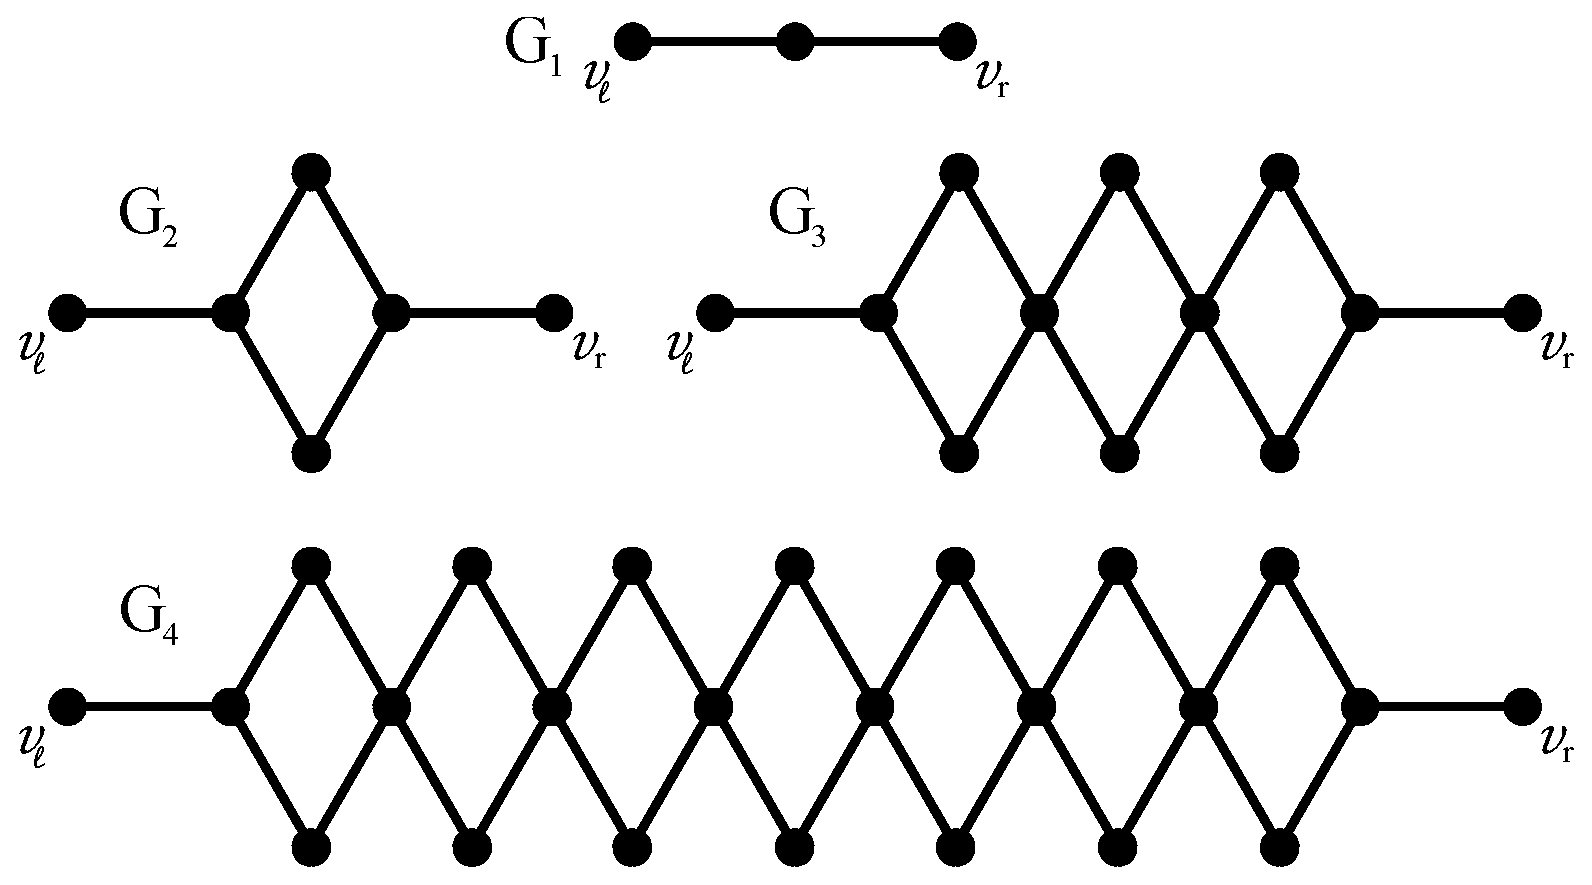
\includegraphics[scale=0.3]{figs/concertina}
  \end{figure}
  \vfill
  Theorem: The VC-dimension of $(\mathbb{S}_{G_i}, F)$ is
  $\lfloor\log_2\mathsf{VD}(G) -2\rfloor +1=i$
  \vfill
  Proof Intuition: The middle vertices are internal to a lot of SPs
\end{frame}

\begin{frame}
  \frametitle{Is the Vertex-Diameter the right quantity?}
  No! If $G$ undirected and for every connected pair of nodes there is a
  unique SP, then the VC-dimension is at most 3\\
  \quad These graphs are not just trees!
  \vfill
  Proof: in such a graph, two SPs that meet and separate can not meet again\\
  \quad (+ multiple case analysis)
  \vfill
  The bound ``3'' is tight. In the following graph we can shatter 3 paths
  \begin{figure}[H]
    \centering
    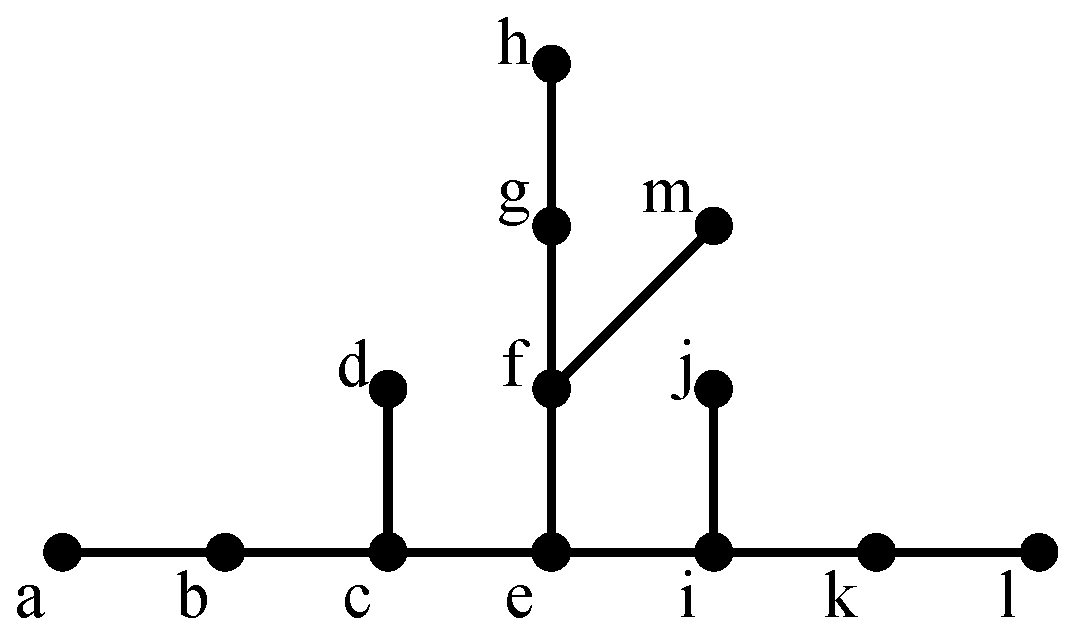
\includegraphics[scale=0.3]{figs/uniqueshortestpathtight}
  \end{figure}
  \vfill
  There is room for improvement using pseudodimension (we are working on that!)
\end{frame}

\begin{frame}
  \frametitle{What about directed graphs?}
  Does a similar result also hold for directed graphs with unique SP?\\
  \quad  Not for the same constant $3$. We built a graph with unique SPs between
  all connected nodes and we can shatter a set of $4$ SPs
  \begin{figure}[H]
    \centering
    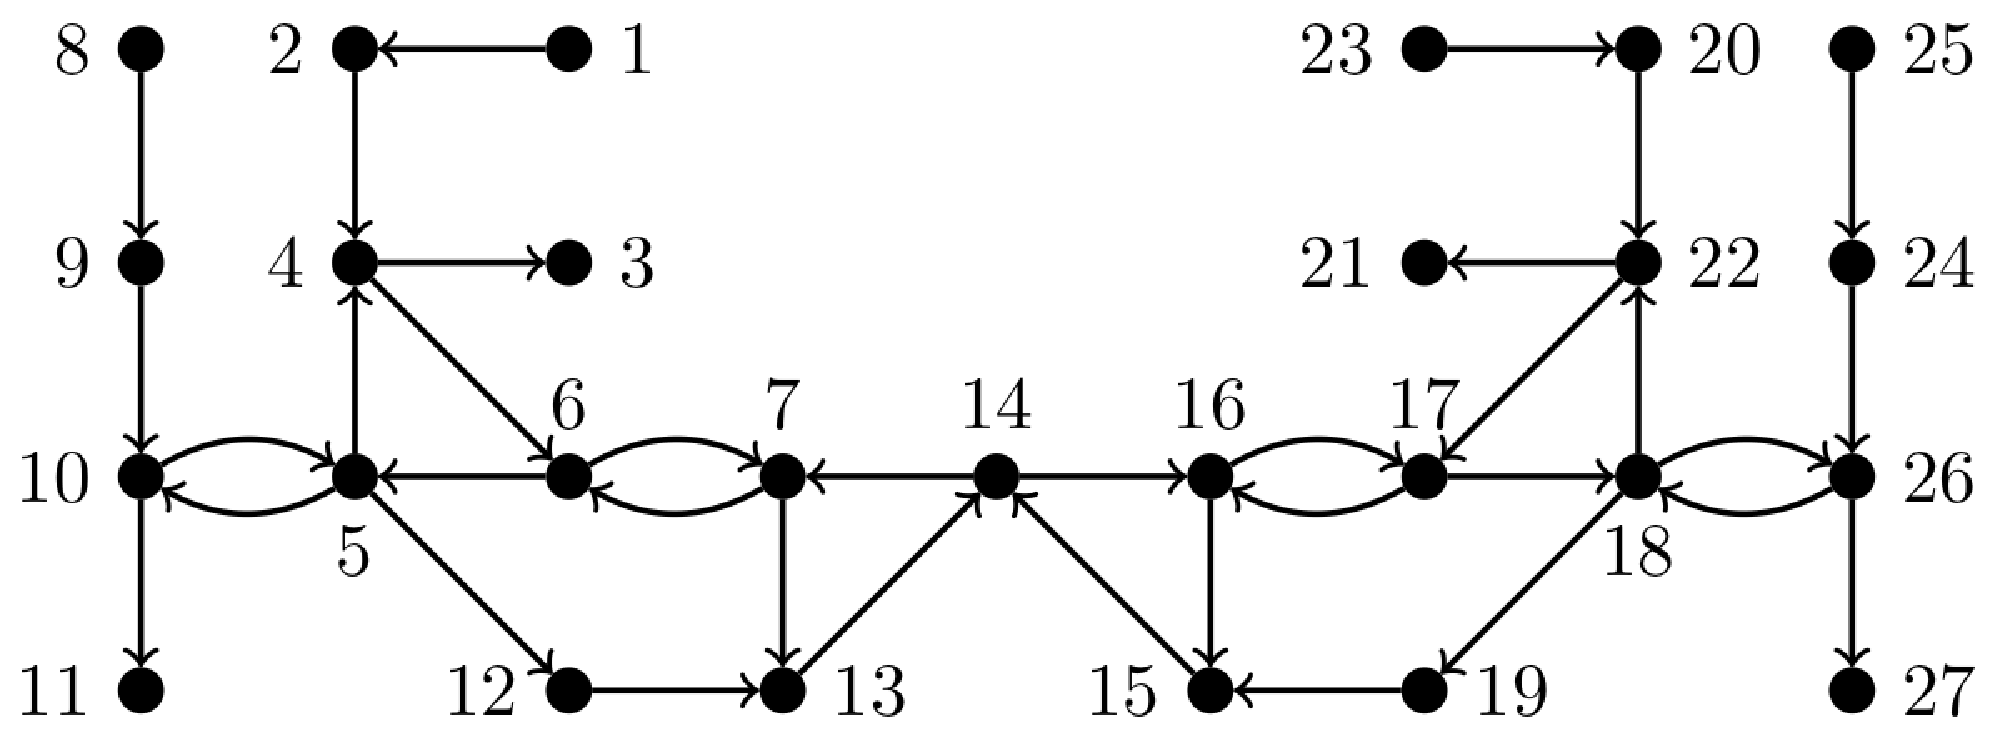
\includegraphics[scale=0.3]{figs/uniquedirected}
  \end{figure}
  Yes, finding counterexamples is messy\ldots
  \vfill
  Does it hold for a different constant?\\
  \quad We do not know! Maybe you can work on that?
\end{frame}

\begin{frame}
  \frametitle{How well does the algorithm perform in practice?}
  It performs very well!
  \vfill
  We tested the algorithm on real graphs (SNAP) and on artificial
  Barabasi-Albert graphs, to evalue its accuracy, speed, and scalability
  \vfill
  Results: It blows away the exact algorithm and the union-bound-based
  sampling algorithm
\end{frame}

\begin{frame}
  \frametitle{How accurate is the algorithm?}
  In $O(10^3)$ runs of the algorithm on different graphs and with different
  parameters, we always had $|\tilde{\betw}(v)-\betw(v)|<\varepsilon$ for all
  nodes\\
  \quad Actually, on average $|\tilde{\betw}(v)-\betw(v)|<\varepsilon/8$
  \vfill
  \begin{figure}[H]
    \centering
    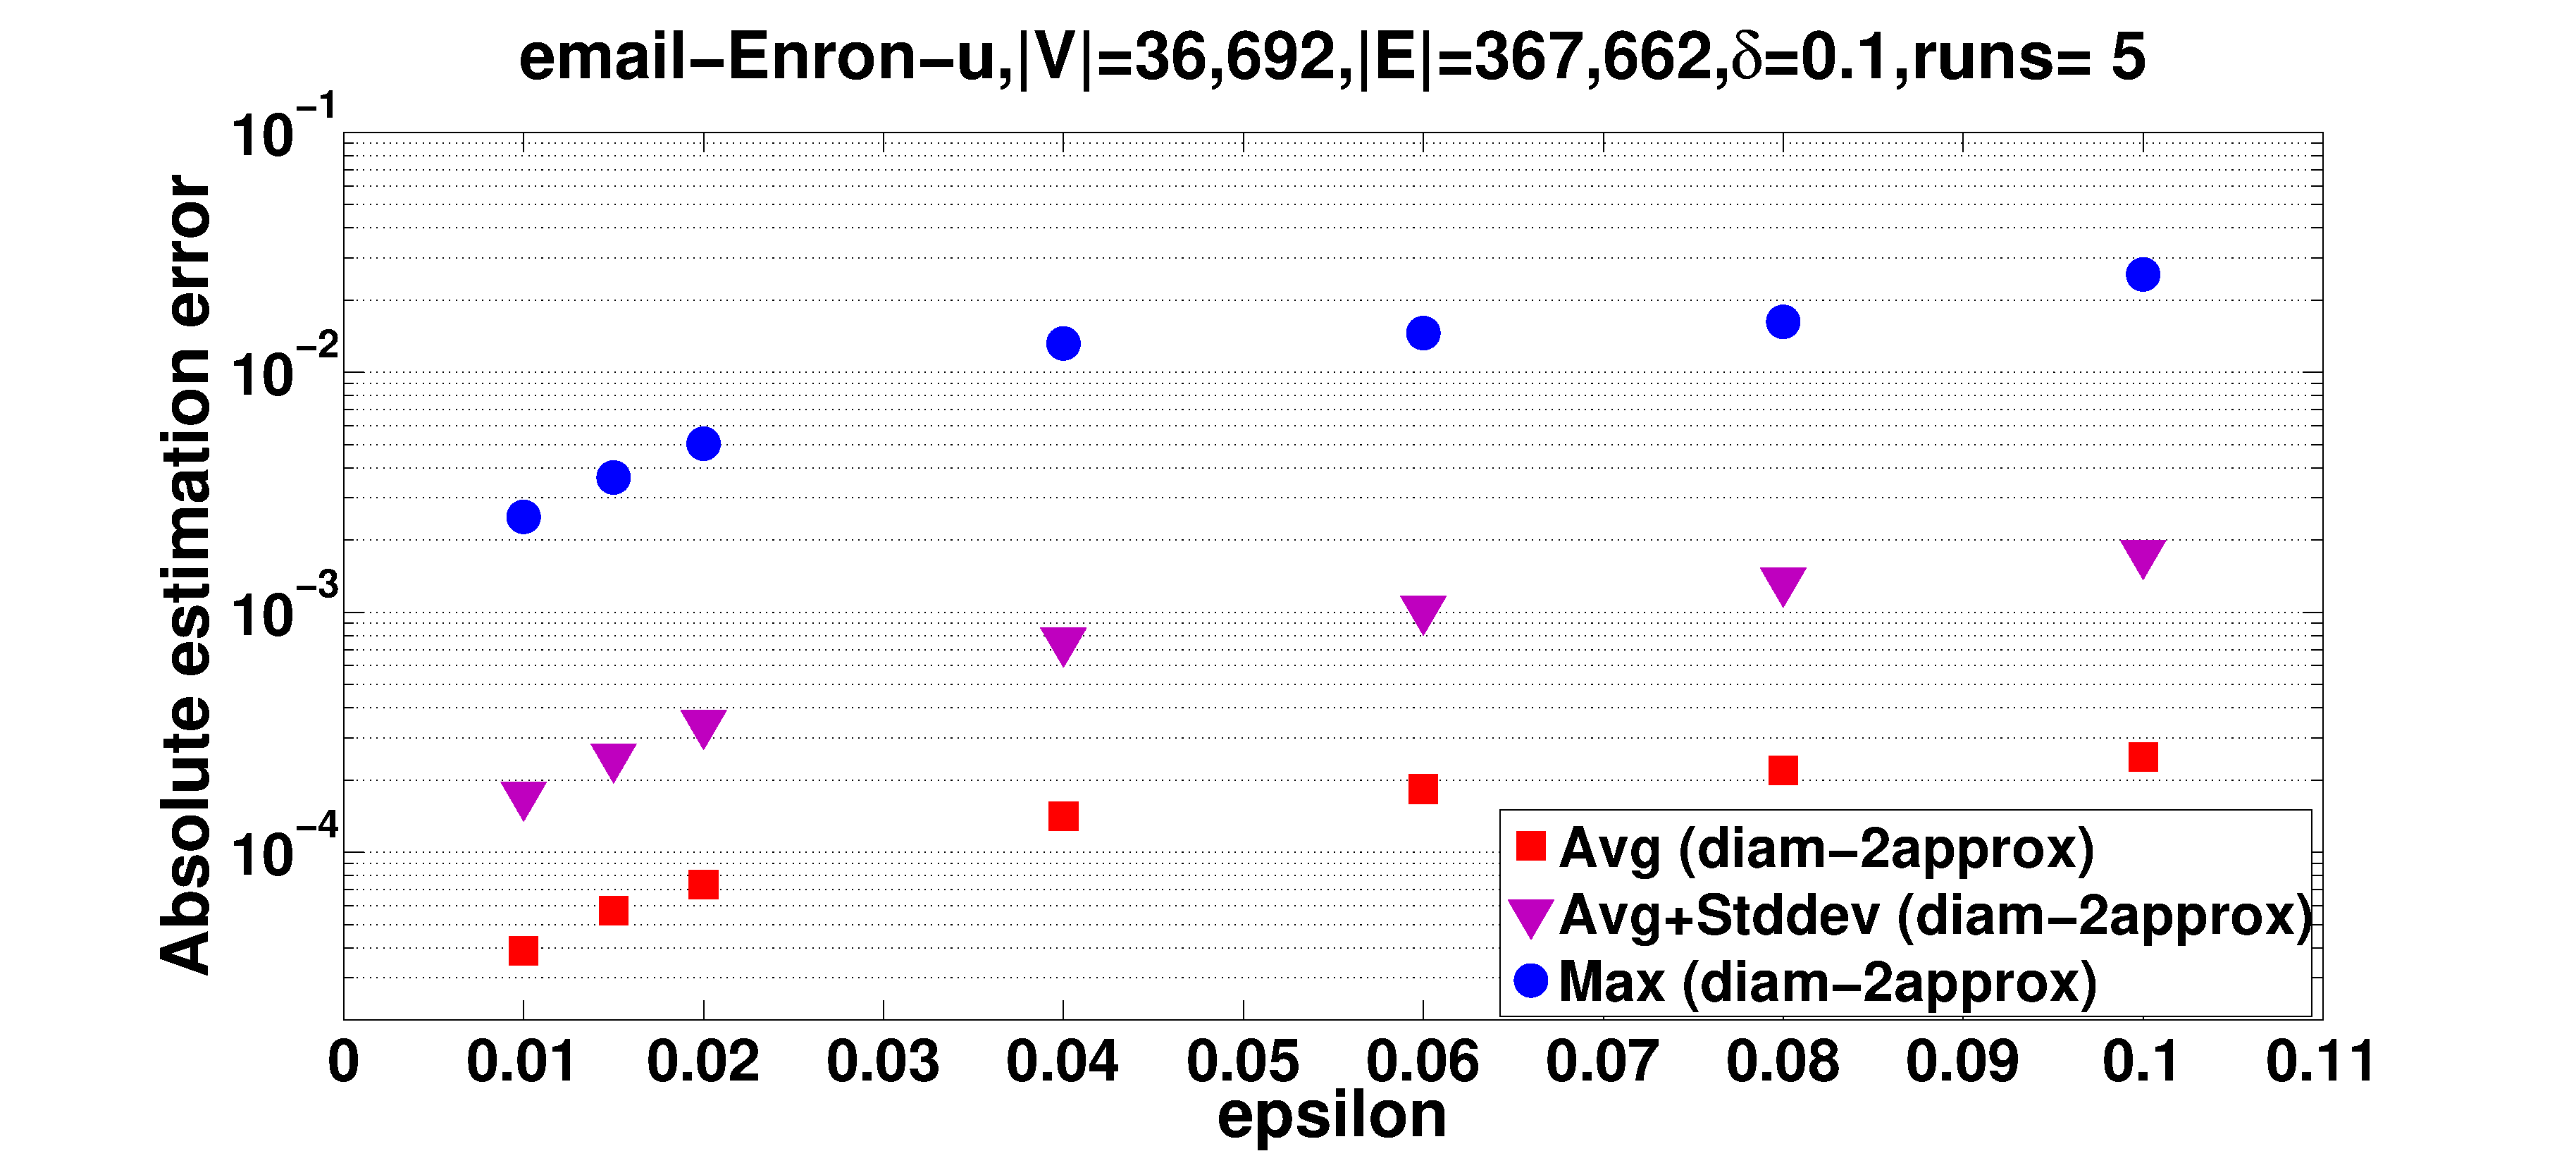
\includegraphics[scale=0.22]{figs/email-Enron-error}
  \end{figure}
\end{frame}

\begin{frame}
  \frametitle{How fast is the algorithm?}
  Approximately 8 times faster than the simple sampling algorithm
  \vfill
  Variable speedup w.r.t. exact algorithm (200x -- 4x), depending on
  $\varepsilon$
  \vfill
  \begin{figure}[H]
    \centering
    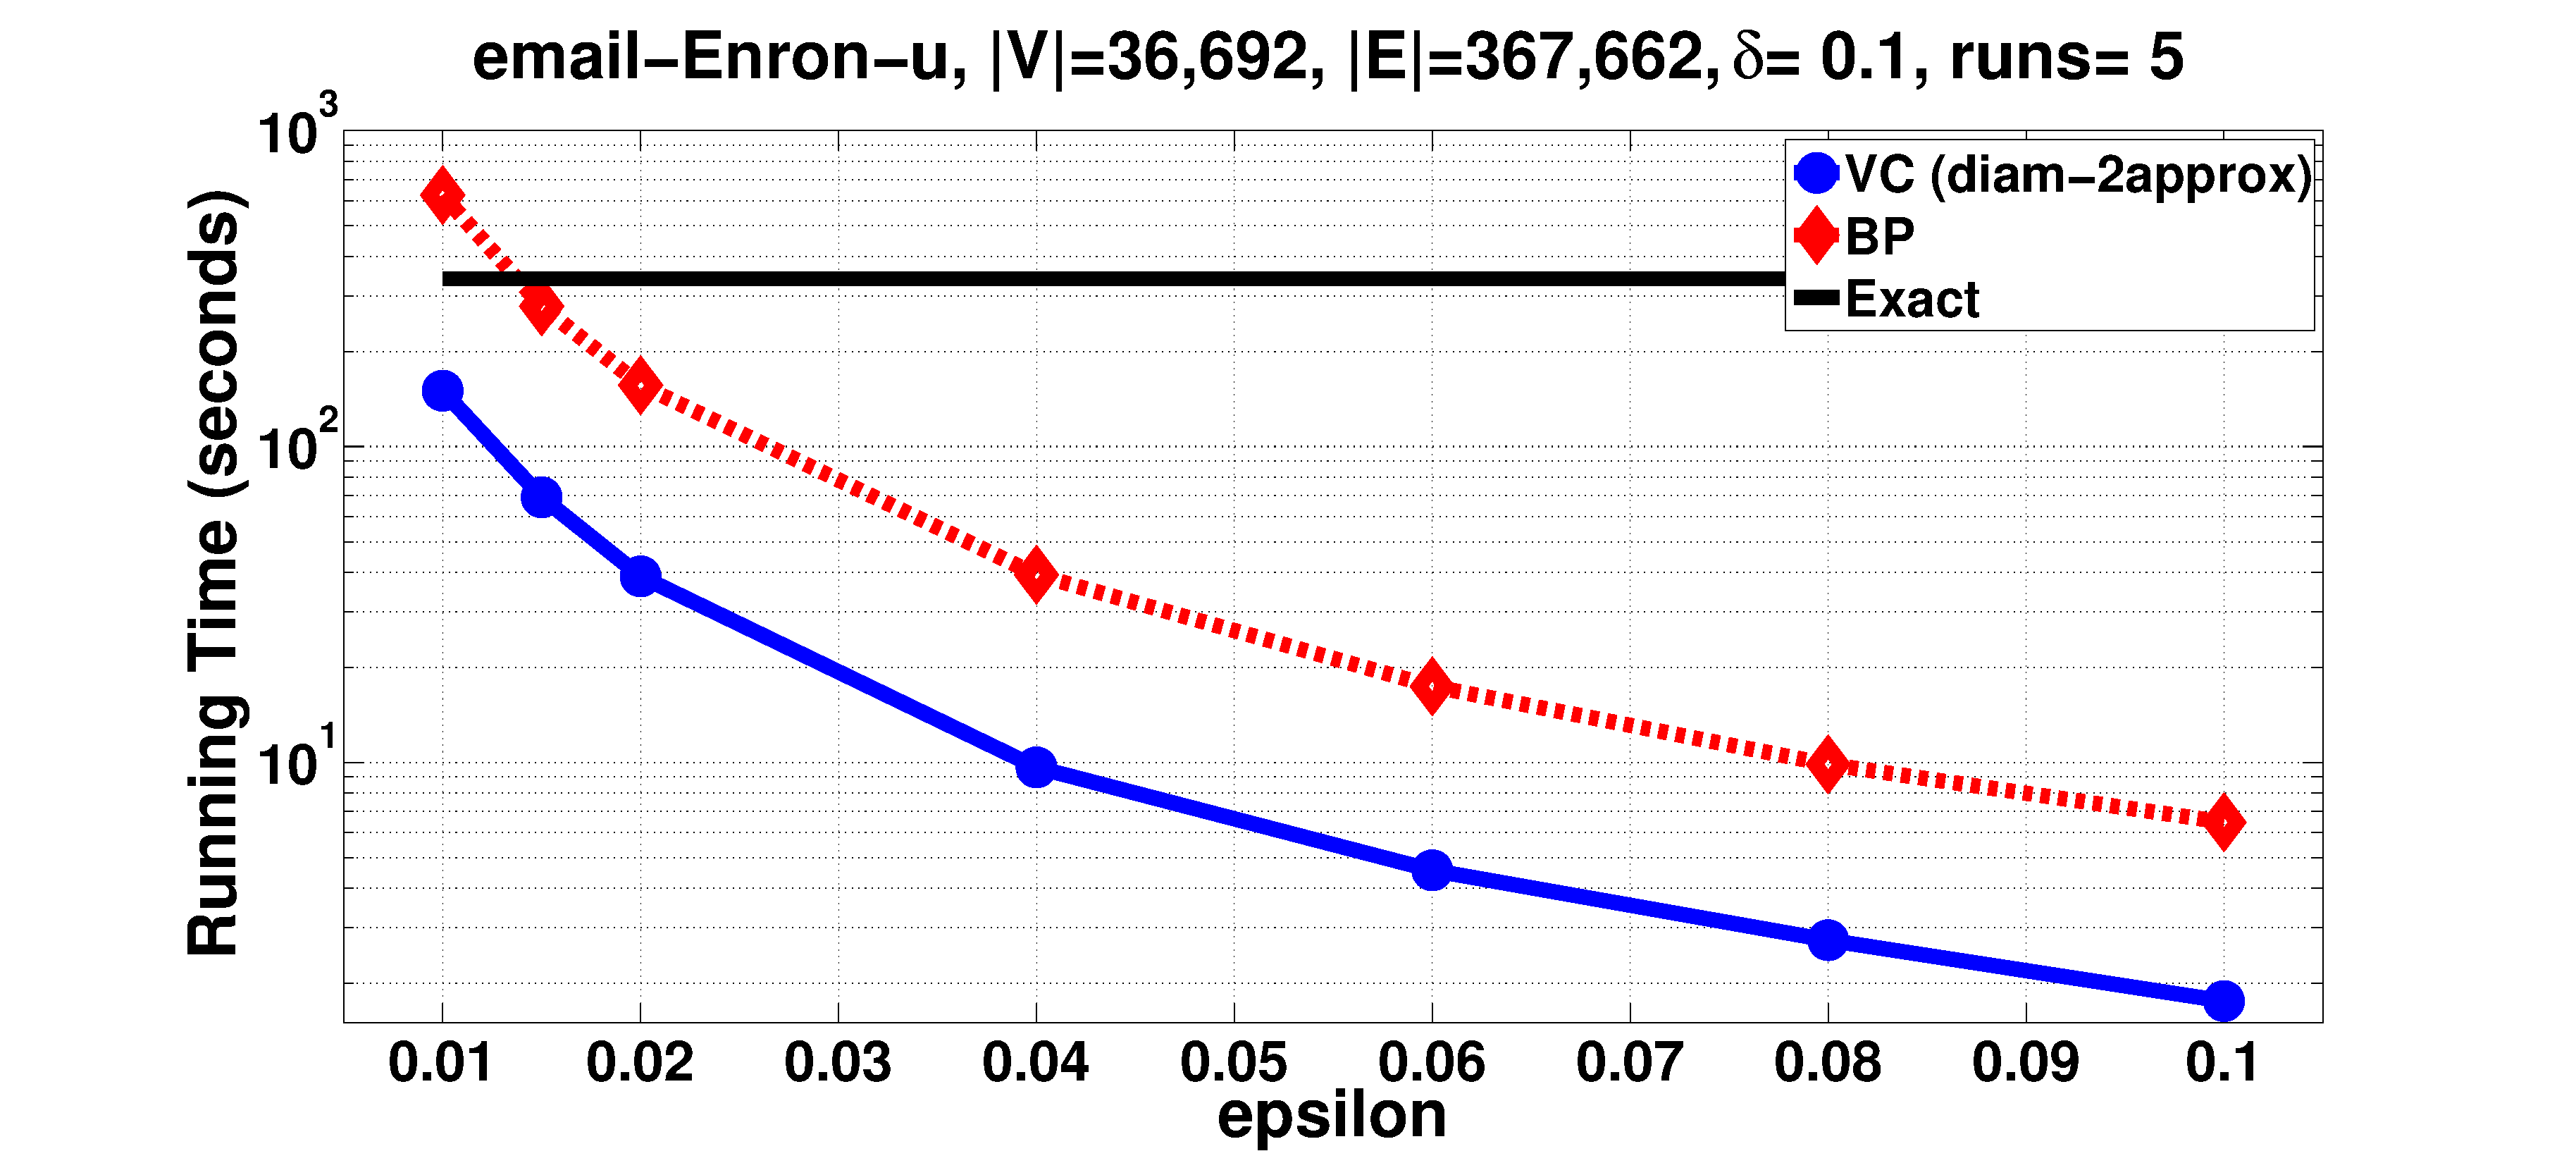
\includegraphics[scale=0.22]{figs/email-Enron-time}
  \end{figure}
\end{frame}

\begin{frame}
  \frametitle{How scalable is the algorithm?}
  Much more scalable than the simple sampling algorithm, because the sample
  size does not depend on $n$
  \vfill
  \begin{figure}[H]
    \centering
    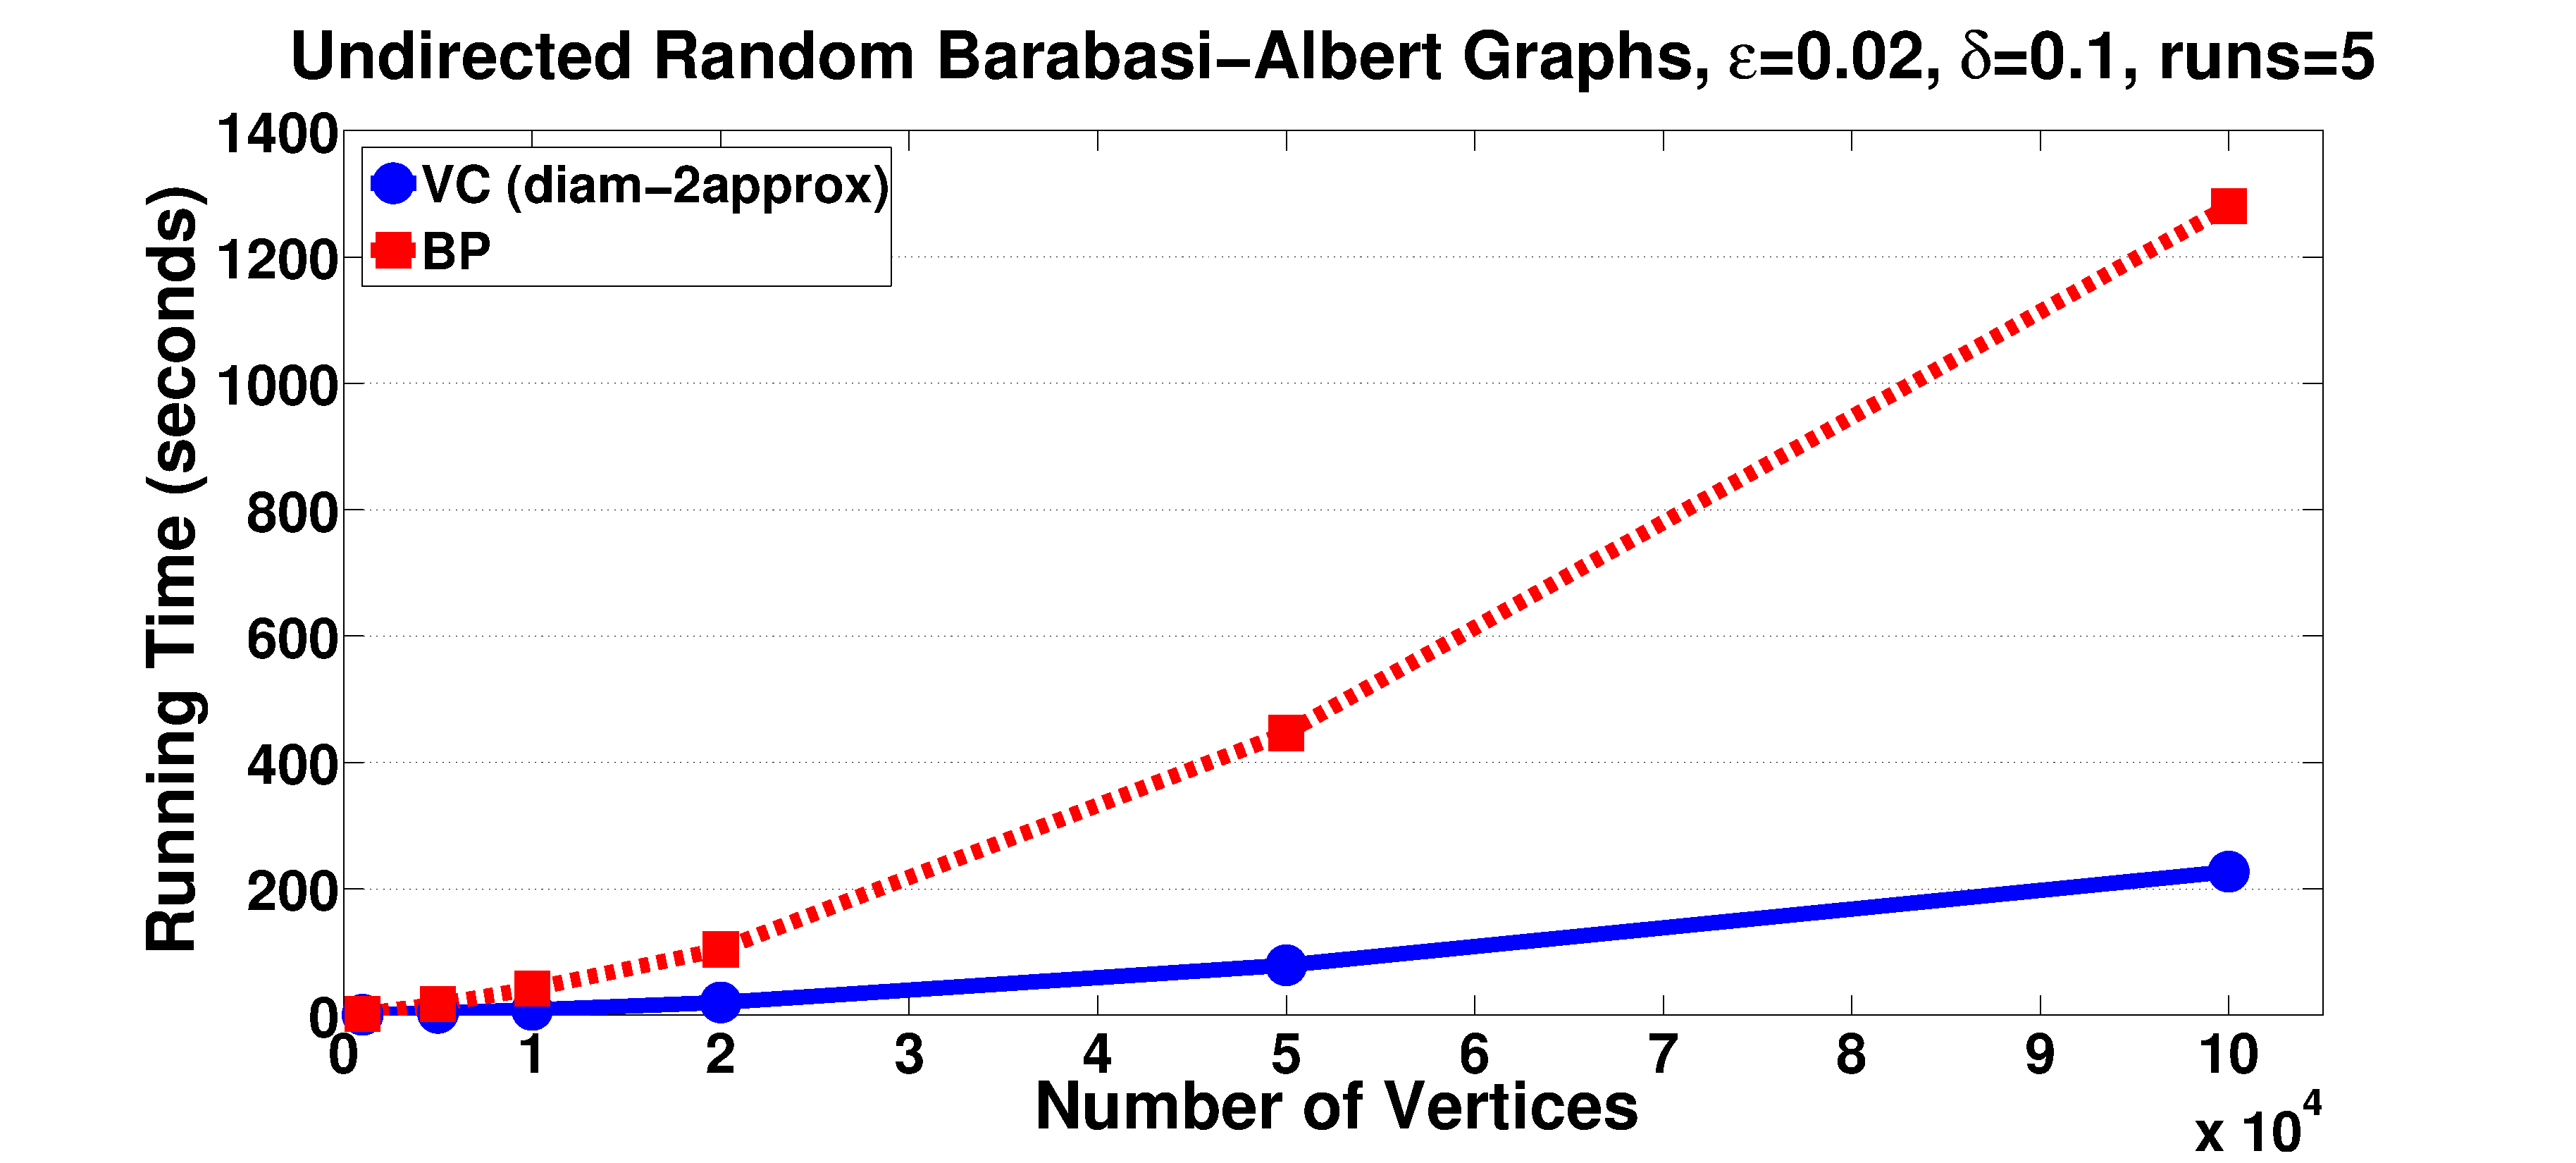
\includegraphics[scale=0.22]{figs/random-time}
  \end{figure}
\end{frame}

\begin{frame}
  \frametitle{Conclusions (Betweenness Centrality)}
  \vfill
  We showed a sampling algorithm for betweenness centrality approximation that
  gives probabilistic guarantees on the quality of the approximation for all
  the vertices
  \vfill
  The algorithm samples SPs according to a well-defined distribution, and
  the analysis relies on VC-dimension, which is bounded by the Vertex Diameter,
  a characteristic quantity of the graph that is small in real networks
  \vfill
  The use of VC-dimension makes the algorithm much faster and more scalable
  than previous sampling approaches and than the exact algorithm
\end{frame}

% !TEX root =  centrtutorial.tex
\begin{frame}
  \frametitle{Betweenness Centrality ? Incremental and Faster}
  \centering
  \vfill
  {\huge Meghana Nasre, Matteo Pontecorvi, Vijaya Ramachandran}
  \vfill
  {\large MFCS '14: Mathematical Foundations of Computer Science}
\end{frame}

\begin{frame}
  \frametitle{Path Dependency}
  
  \begin{itemize}
    \item Pair dependency of $(s,w)$ on $v$:
      \[\dep_{st}(w)=\frac{\paths_{sw}(v)}{\paths_{sw}}\]
    \item Dependency of a node $s$ on another node $v$:
      \[\dep_s(v)=\sum_{t \in V}\dep_{st}(w)\]
    \item Can be computed recursively:
    \[
    \dep_s(v)=\sum_{w \mid v \in \pred_s(w) } \frac{\paths_{sv}}{\paths_{sw}} \left( 1 + \dep_{s}(w) \right)
    \]
    \item Betweenness can be expressed as function of dependencies:
      \[ \betw(v) = \sum_{s \neq v} \dep_s(v) \]
  \end{itemize}
  
  \begin{figure}[H]
    \centering
    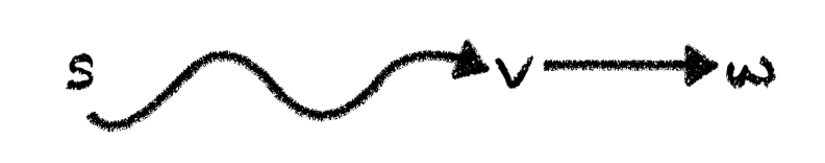
\includegraphics[scale=1]{imgs/path-dependency}
  \end{figure}
  
\end{frame}

\begin{frame}
  \frametitle{Main Result}

  \begin{figure}[H]
    \centering
    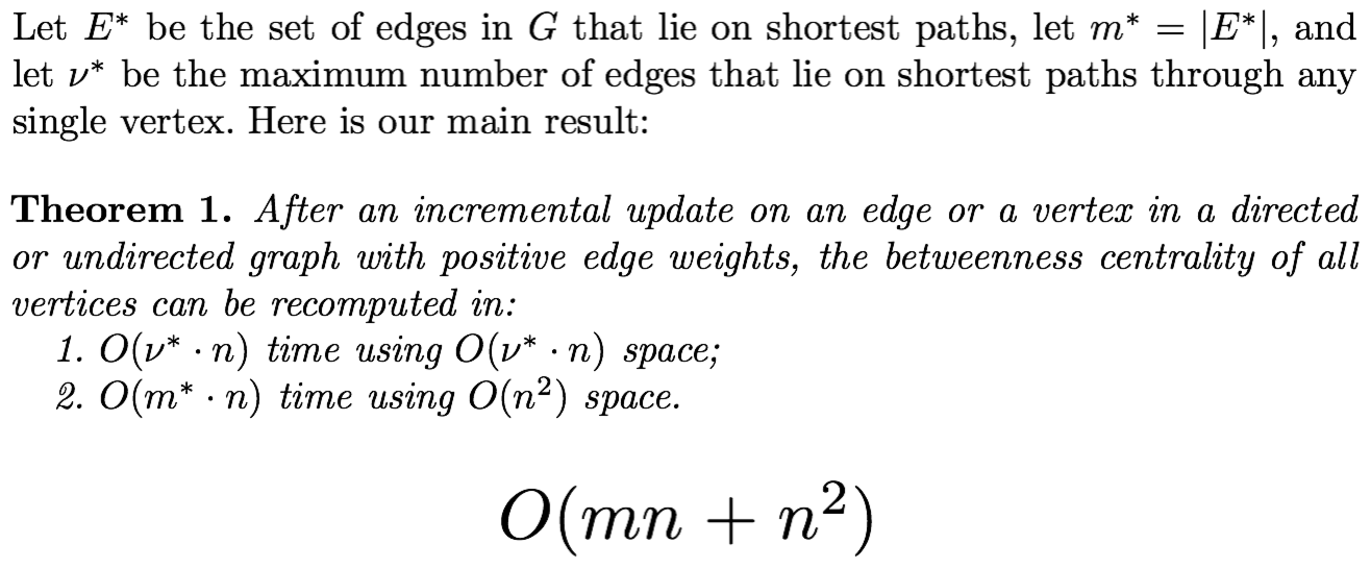
\includegraphics[width=\textwidth]{imgs/npr14-main-result}
  \end{figure}
  
\end{frame}

\begin{frame}
  \frametitle{Lemmas}

  \begin{figure}[H]
    \centering
    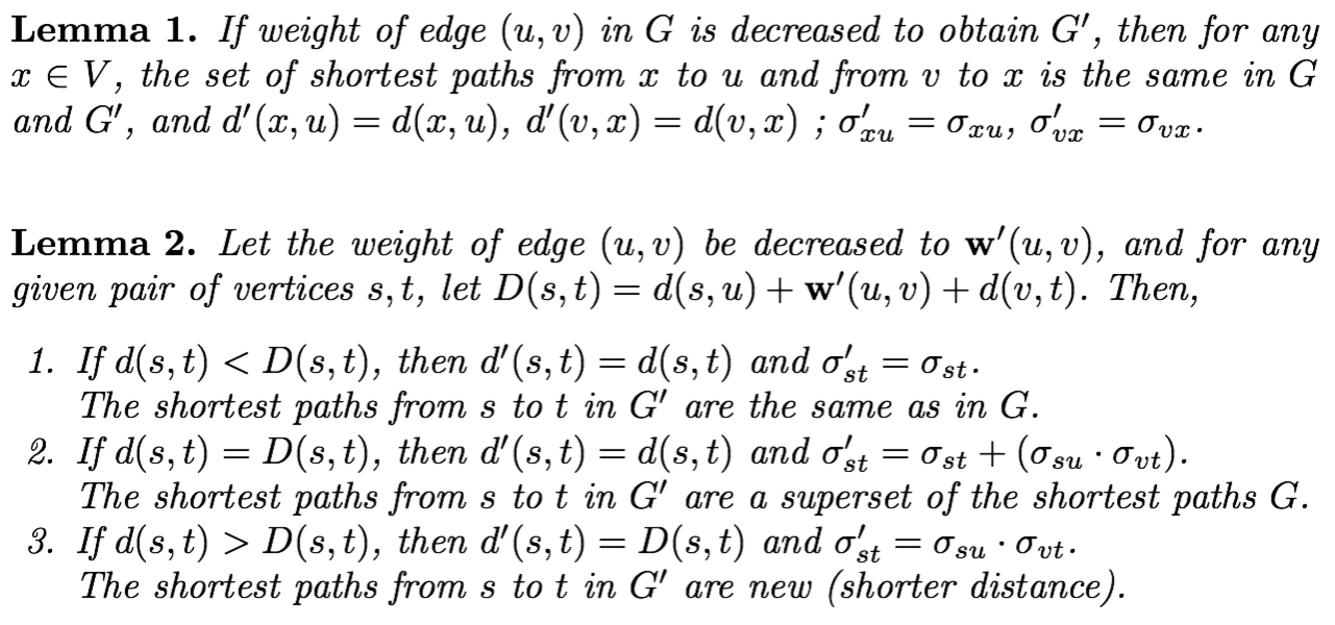
\includegraphics[width=\textwidth]{imgs/npr14-lemmas}
  \end{figure}
  
\end{frame}

\begin{frame}
  \frametitle{SSSP DAG Update}

  \begin{figure}[H]
    \centering
    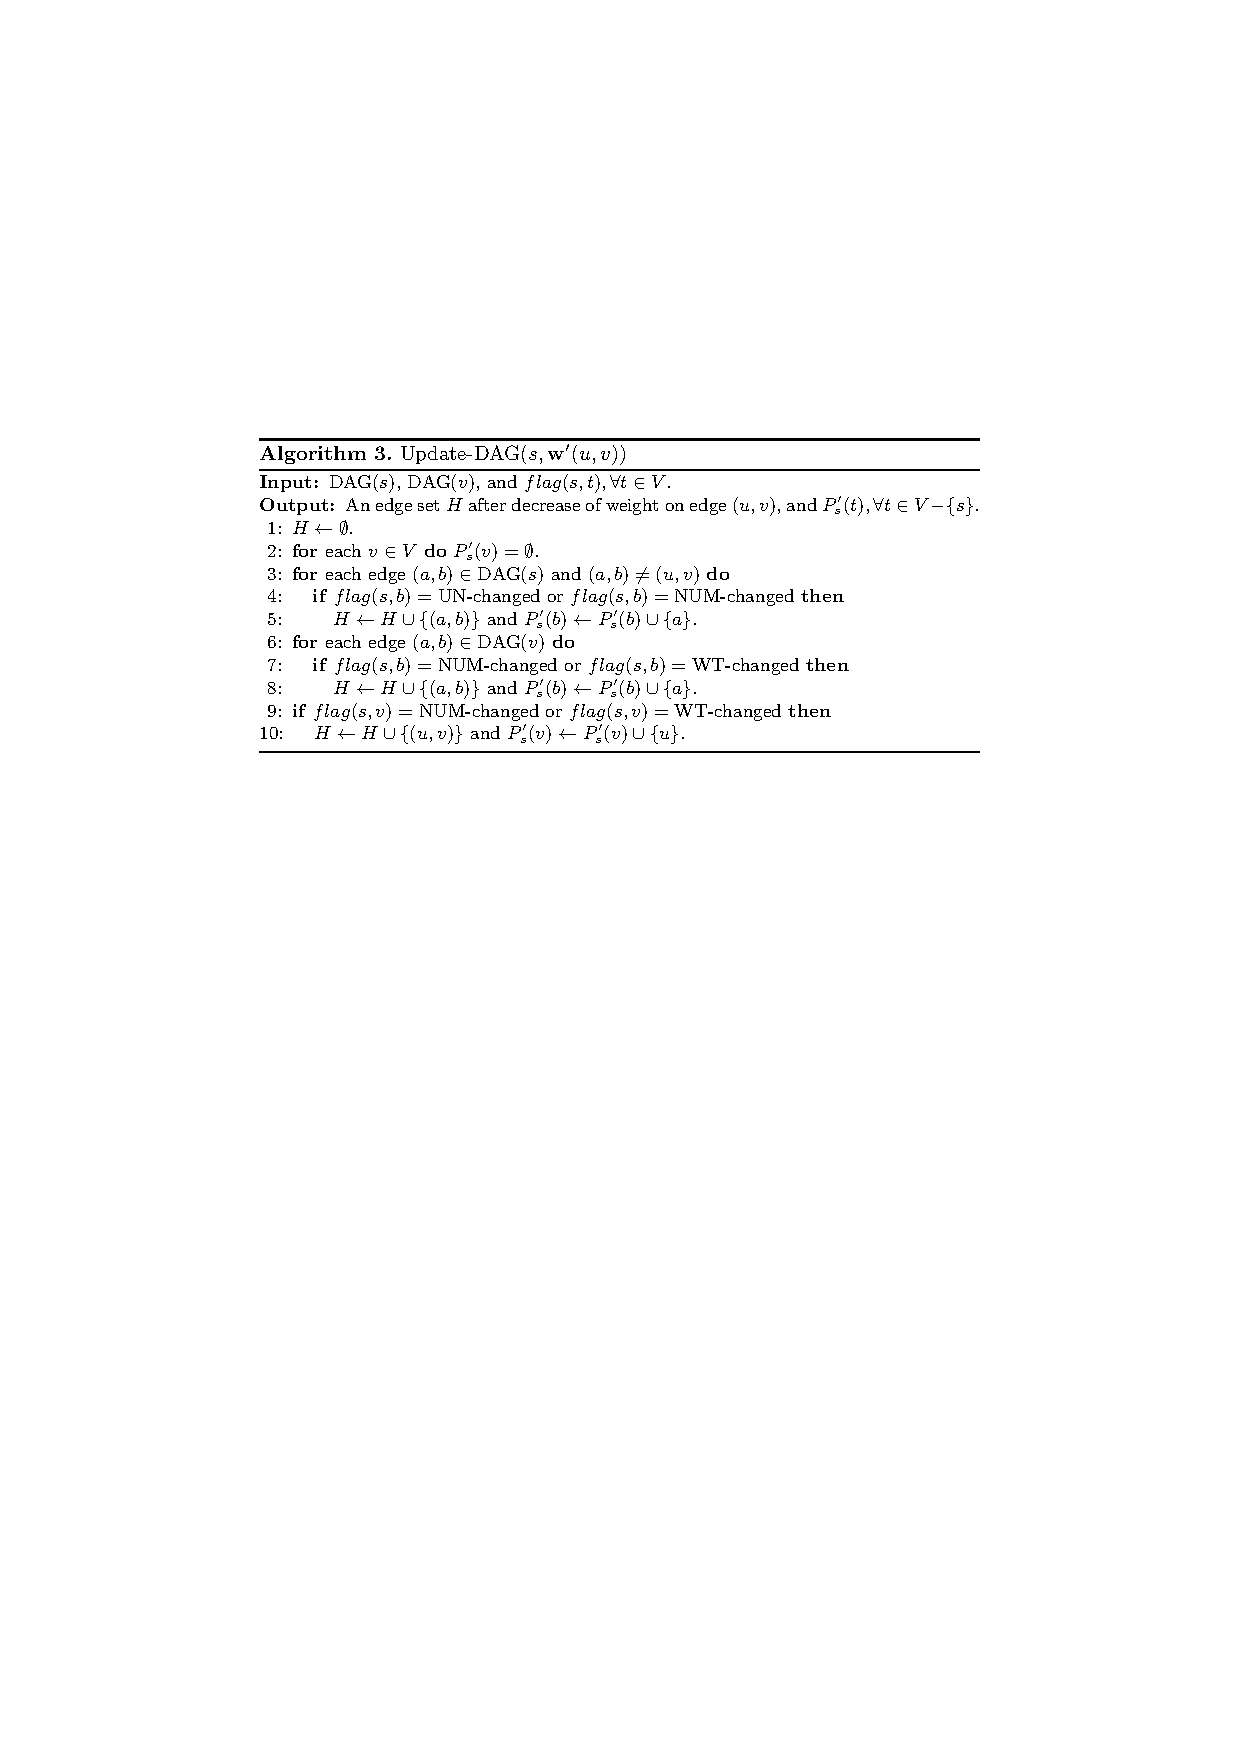
\includegraphics[width=\textwidth]{imgs/npr14-algo3}
  \end{figure}
  
\end{frame}

\begin{frame}
  \frametitle{Edge Update}

  \begin{figure}[H]
    \centering
    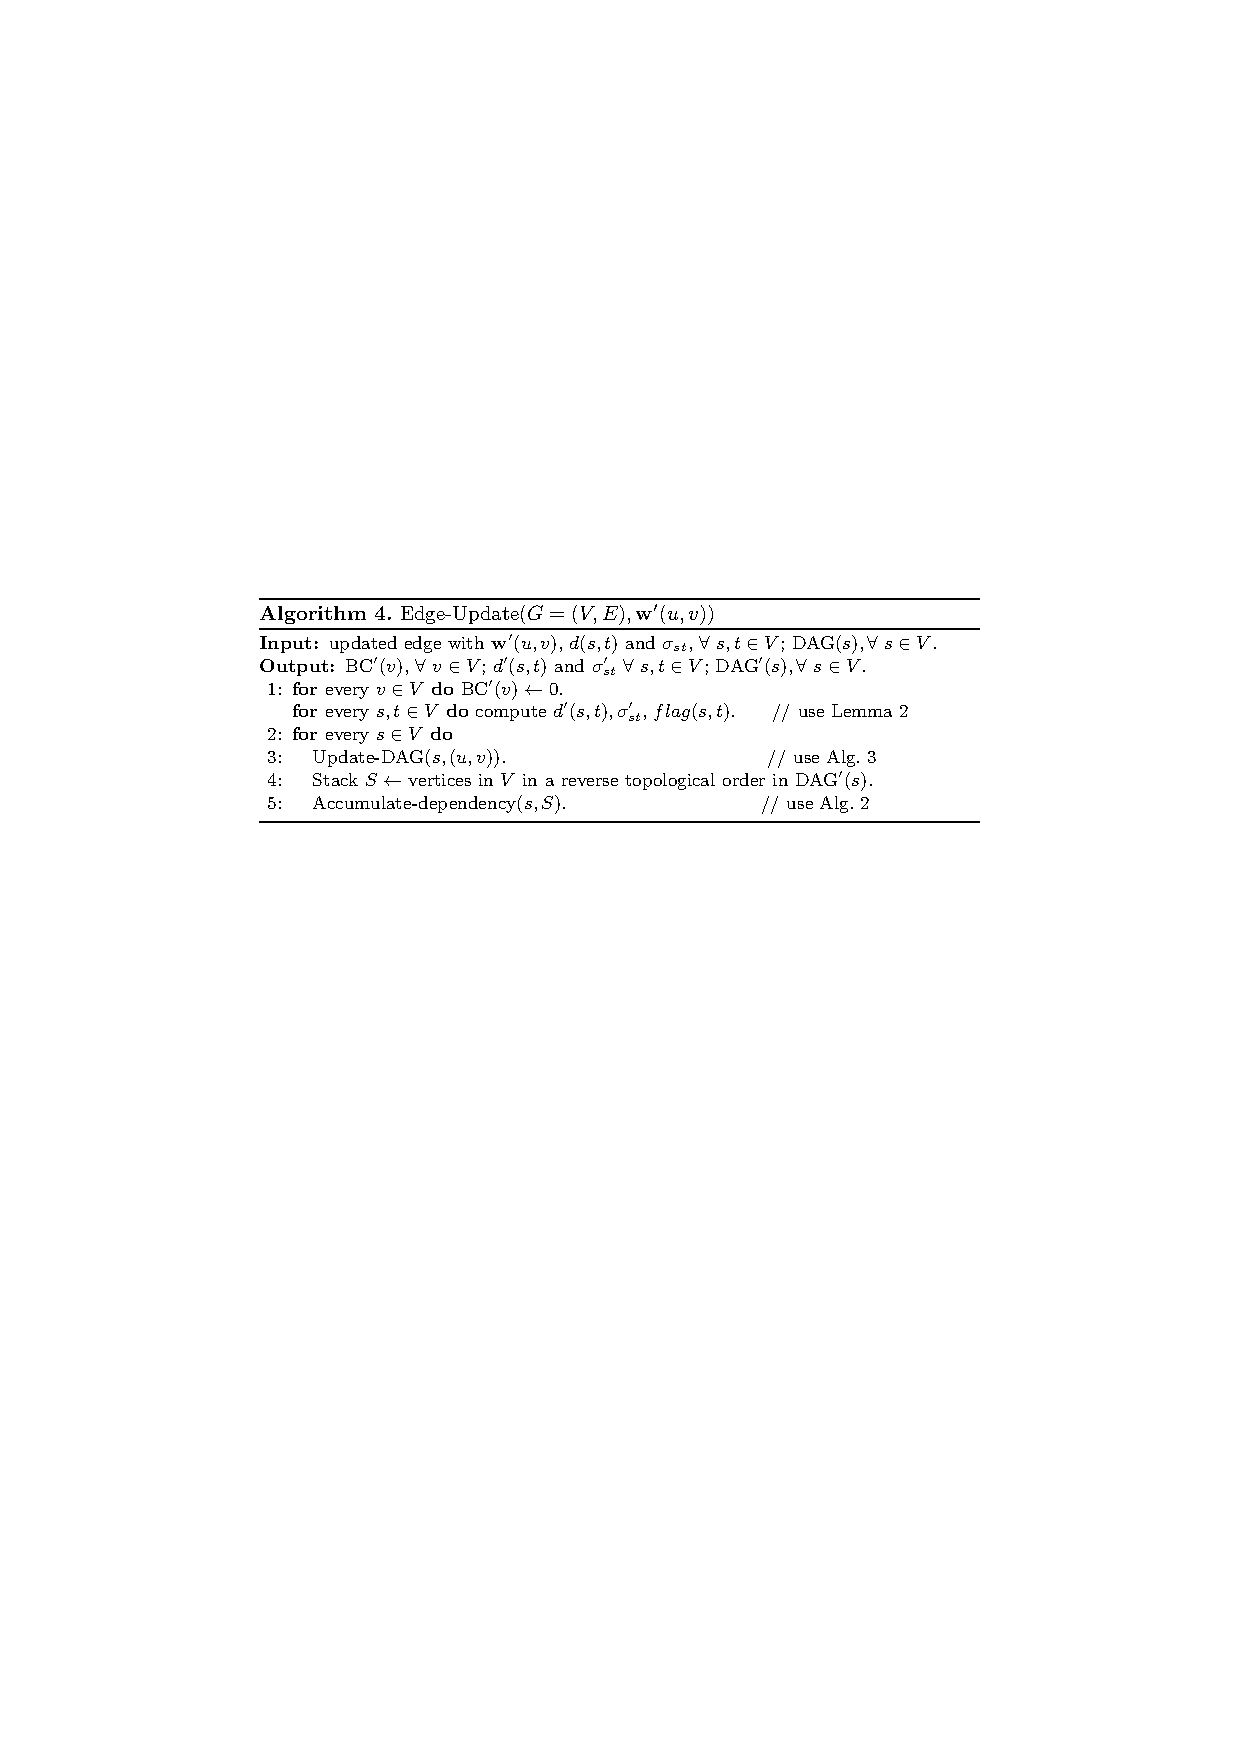
\includegraphics[width=\textwidth]{imgs/npr14-algo4}
  \end{figure}
  
\end{frame}

\begin{frame}
  \frametitle{Space-Efficient Variant $O(n^2)$}
  
  \begin{itemize}
    \item Do not store the \sssp \dag
    \item Store only $E^*$
    \item Updated \dag can be build in $O(m^*)$ time
    \begin{itemize}
      \item Time $O(m^* \times n)$
      \item Compute ${E'}^*$ from $E^*$, then $\dag'(s)$ from ${E'}^*$
    \end{itemize}
    \item Space $O(m^* + n^2)$ to store $E^*$ and $n^2$ distances $\dist(s,t)$ and shortest paths $\paths_{st}$
  \end{itemize}
  
\end{frame}

\begin{frame}
  \frametitle{Comparison}

  \begin{figure}[H]
    \centering
    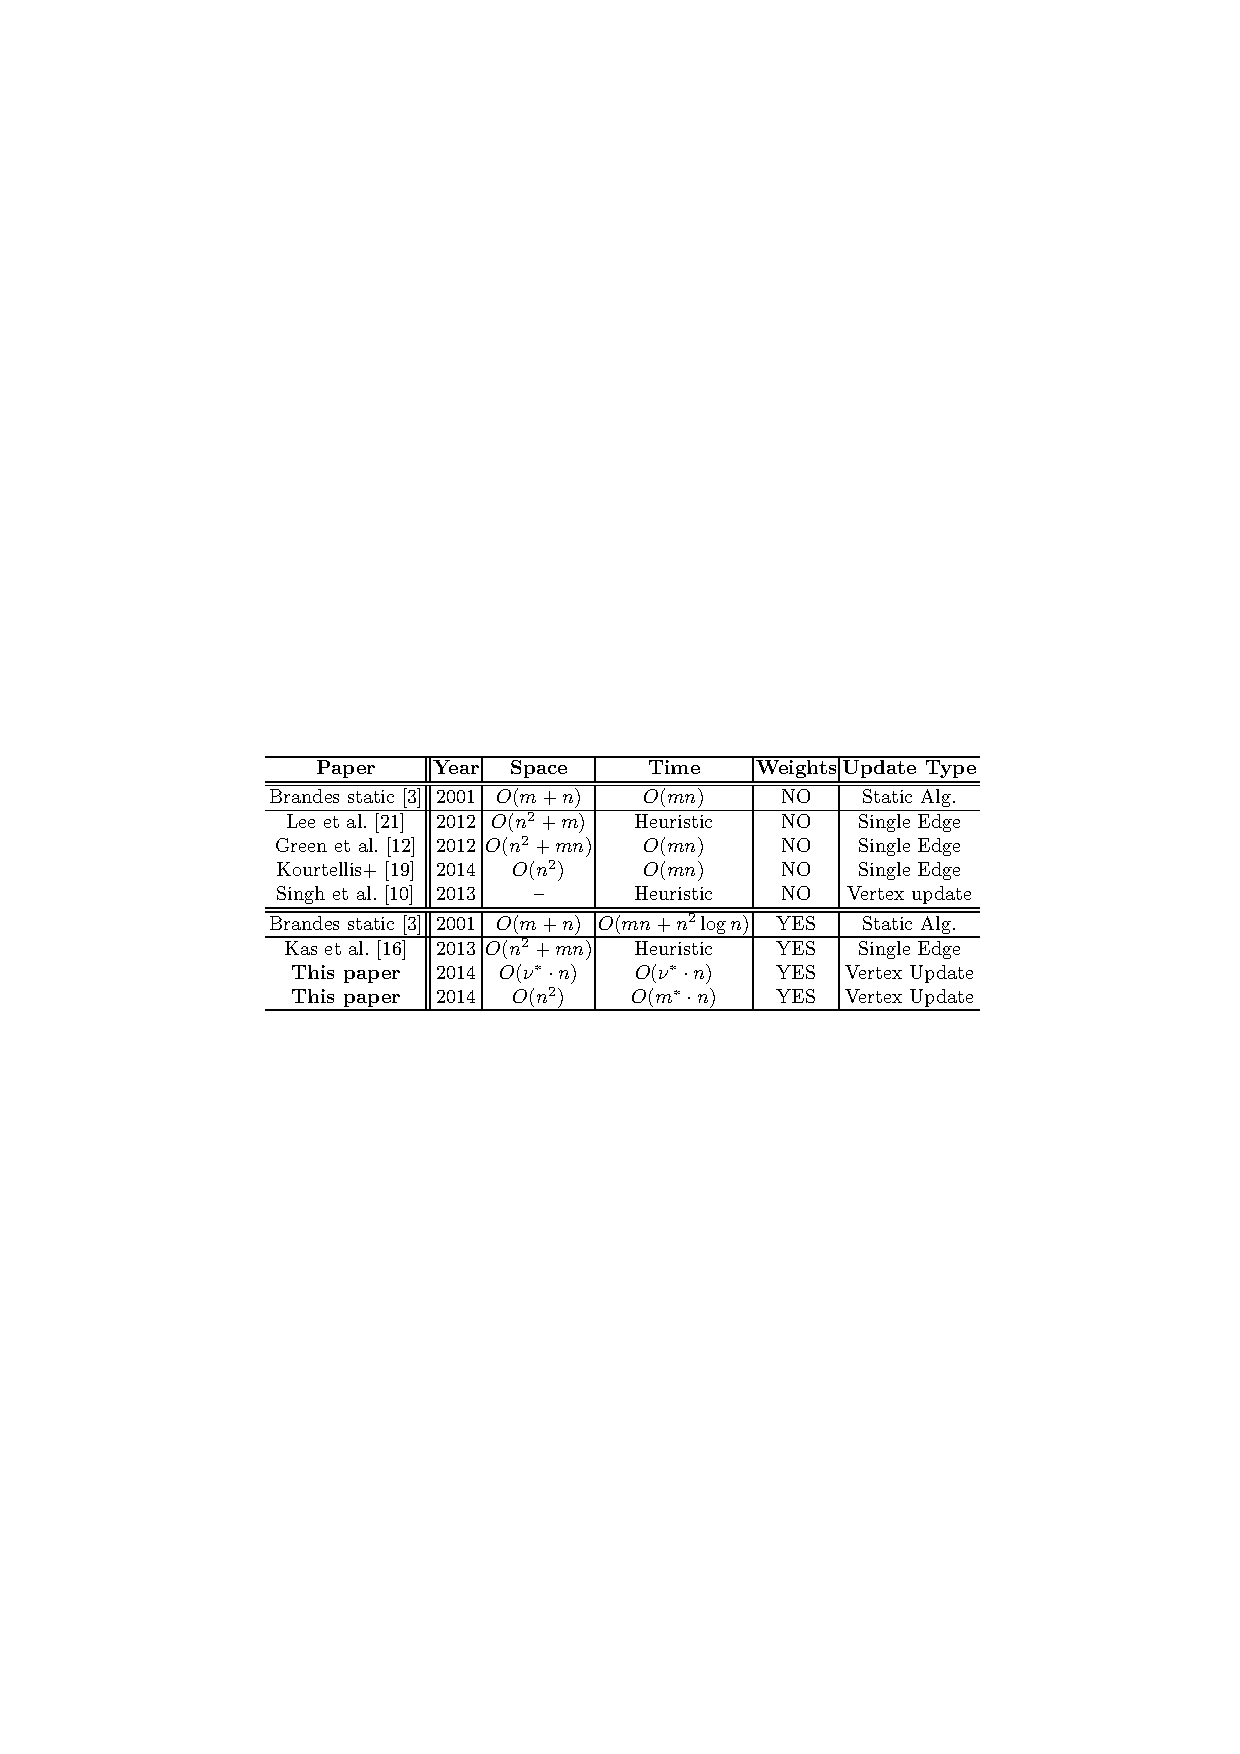
\includegraphics[width=\textwidth]{imgs/npr14-comparison}
  \end{figure}
  
\end{frame}

\begin{frame}
  \frametitle{Shortcomings}

  \begin{itemize}
    \item Not fully dynamic (no edge removal)
    \item $m^*$ can be large in practice
    \item Non-trivial to parallelize (need to access pairs of \sssp \dag at a time)
    \item Does not solve main bottleneck of most algorithms: $O(n^2)$ memory
  \end{itemize}
  
\end{frame}

\end{document}
